% This is file JFM2esam.tex
% first release v1.0, 20th October 1996
%       release v1.01, 29th October 1996
%       release v1.1, 25th June 1997
%       release v2.0, 27th July 2004
%       release v3.0, 16th July 2014
%   (based on JFMsampl.tex v1.3 for LaTeX2.09)
% Copyright (C) 1996, 1997, 2014 Cambridge University Press

\documentclass{jfm}
\usepackage{graphicx}
\usepackage{epstopdf, epsfig}
\usepackage{amsmath}
\usepackage{amsfonts}
\newtheorem{lemma}{Lemma}
\newtheorem{corollary}{Corollary}

% our colors
\usepackage[usenames,dvipsnames]{xcolor}
\colorlet{cesar}{red}
\colorlet{greg}{green}
\colorlet{bill}{blue}

% copy-editing printing
% \usepackage{geometry}
% \geometry{a4paper,left=5.25cm,right=5 .25cm,top=3.5cm,bottom=3.5cm}
% \linespread{1.}
% \usepackage{multicol}


% our packages
\usepackage{showlabels}

% hyperref
\usepackage{hyperref}
\hypersetup{
        %draft,
        breaklinks=true,
        colorlinks=true,
        linkcolor=blue,
        citecolor=Purple,
        urlcolor=Purple,
        pdfstartview={FitH},
        pdfview={FitH 0},
        pdfauthor={Cesar B. Rocha},
        pdftitle={NIWs extract energy from barotropic quasigeostrophic flow},
 }


%\shorttitle{ Extraction of  energy from barotropic turbulence by near-inertial waves}
\shorttitle{Near-inertial waves extract energy from barotropic quasigeostrophic flow}

\shortauthor{Cesar B. Rocha, Gregory L. Wagner, and William R Young}

%\title{Extraction of energy from barotropic turbulence by near-inertial waves:
%        freely-evolving flow}

\title{Near-inertial waves extract energy from barotropic quasigeostrophic flow}
\author{Cesar B. Rocha\aff{1}
  \corresp{\email{crocha@ucsd.edu}},
  Gregory L. Wagner\aff{2}
 \and William R. Young\aff{1}}

\affiliation{\aff{1}Scripps Institution of Oceanography, University of California,
            San Diego
\aff{2}Department of Earth, Atmospheric and Planetary Sciences, Massachusetts
            Institute of Technology}



\begin{document}

\newcommand{\com}{\, ,}
\newcommand{\per}{\, .}

%% Averages
% Use \bar to over line solo symbols

\newcommand{\av}[1]{\bar{#1}}
\newcommand{\avbg}[1]{\overline{#1}}
\newcommand{\avbgg}[1]{\overline{#1}}

% A nice definition
\newcommand{\defn}{\ensuremath{\stackrel{\mathrm{def}}{=}}}

% space in equations
\newcommand{\qqand}{\qquad \text{and} \qquad}
\newcommand{\qand}{\quad \text{and} \quad}

% equations
\def\beq{\begin{equation}}
\def\eeq{\end{equation}}

\def\bea{\begin{align}}
\def\ena{\end{align}}


% calculus
\newcommand{\ord}{\mathcal{O}}
%\newcommand{\p}{\partial}
\newcommand{\ii}{{\rm i}}
\newcommand{\dd}{{\rm d}}
\newcommand{\id}{{\, \rm d}}
\newcommand{\ee}{{\rm e}}
\newcommand{\DD}{{\rm D}}
\newcommand{\wavy}{\text{wavy}}
\newcommand{\qg}{\text{qg}}
\newcommand{\dt}{\Delta t}
\newcommand{\dx}{\Delta x}
\newcommand{\be}{\beta}

\newcommand{\al}{\alpha}
\newcommand{\bx}{\boldsymbol{x}}
\newcommand{\by}{\boldsymbol{y}}
\newcommand{\bu}{\boldsymbol{u}}
\newcommand{\bv}{\boldsymbol{v}}


\newcommand{\half}{\tfrac{1}{2}}
\newcommand{\halfi}{\tfrac{\ii}{2}}
\newcommand{\quarter}{\tfrac{1}{4}}
\newcommand{\quarteri}{\tfrac{\ii}{4}}
\newcommand{\halfrho}{\tfrac{1}{2}}
\newcommand{\rz}{{}}
\newcommand{\bn}{\boldsymbol{\hat n}}
\newcommand{\br}{\boldsymbol{r}}
\newcommand{\bR}{\boldsymbol{R}}
\newcommand{\bA}{\ensuremath {\boldsymbol {A}}}
\newcommand{\bB}{\ensuremath {\boldsymbol {B}}}
\newcommand{\bU}{\ensuremath {\boldsymbol {U}}}
\newcommand{\bE}{\ensuremath {\boldsymbol {E}}}
\newcommand{\bN}{\ensuremath {\boldsymbol {\mathrm{N}}}}
\newcommand{\bJ}{\ensuremath {\boldsymbol {J}}}
\newcommand{\bXX}{\ensuremath {\boldsymbol {\mathcal{X}}}}
\newcommand{\bFF}{\ensuremath {\boldsymbol {F}}}
\newcommand{\bF}{\ensuremath {\boldsymbol {F}^{\sharp}}}
\newcommand{\bG}{\ensuremath {\boldsymbol G}}
\newcommand{\bSigma}{\ensuremath {\boldsymbol {\Sigma}}}
\newcommand{\bvarphi}{\ensuremath {\boldsymbol {\varphi}}}
\newcommand{\bxi}{\ensuremath {\boldsymbol {\xi}}}
\newcommand{\avbxi}{\overline{\ensuremath {\boldsymbol {\xi}}}}

% math cal

\newcommand{\J}{\mathcal{J}}
\newcommand{\K}{\mathcal{K}}
\newcommand{\cG}{\mathcal{G}}
\newcommand{\cF}{\mathcal{F}}
\newcommand{\cN}{\mathcal{N}}
\newcommand{\cL}{\mathcal{L}}
\newcommand{\cS}{\mathcal{S}}
\newcommand{\cE}{\mathcal{E}}


% san serif for matrices and differential operators
%\newcommand{\helmn}{\mathsf{H}_n}
\newcommand{\helmm}{\triangle_m}
\newcommand{\helmn}{\triangle_n}
\newcommand{\helms}{\triangle_s}
\newcommand{\helm}{\triangle}
\newcommand{\sA}{\mathsf{A}}
\newcommand{\sB}{\mathsf{B}}
\newcommand{\sG}{\mathsf{G}}
\newcommand{\sI}{\mathsf{I}}
%\newcommand{\sJ}{\mathsf{J}}
\newcommand{\sJ}{J}
\newcommand{\gsJ}{\breve{\mathsf{J}}}
\newcommand{\sU}{\mathsf{U}}
\newcommand{\sP}{\mathsf{P}}
\newcommand{\sQ}{\mathsf{Q}}
\newcommand{\sR}{\mathsf{R}}
\newcommand{\sL}{\mathsf{L}}
\newcommand{\Lu}{\mathsf{L}(\what{u}_k)}
\newcommand{\Nu}{\mathsf{N}(\what{u}_k)}
\renewcommand{\L}{\mathsf{L}}
\newcommand{\N}{\mathsf{N}}
\newcommand{\sH}{\mathsf{H}}
\renewcommand{\sI}{\mathsf{I}}
\renewcommand{\L}{\mathsf{L}}
\newcommand{\sM}{\mathsf{M}}
\newcommand{\sT}{\mathsf{T}}
\newcommand{\sGamma}{\mathsf{\Gamma}}
\newcommand{\sOmega}{\mathsf{\Omega}}
\newcommand{\sSigma}{\mathsf{\Omega}}
\newcommand{\sbeta}{\mathsf{\beta}}
\newcommand{\sPi}{\mathsf{\Pi}}
\newcommand{\sC}{\mathsf{C}}
\newcommand{\sQy}{\mathsf{Q}}
\renewcommand{\sb}{\mathsf{b}}

% u
\newcommand{\uhat}{\what{u}_k}

% angle brackets

\def\la{\langle}
\def\ra{\rangle}
\def\laa{\left \langle}
\def\raa{\right \rangle}


%grads and div's
%\newcommand{\bcdot}{\hspace{-0.1em} \boldsymbol{\cdot} \hspace{-0.12em}}
%\newcommand{\bnabla}{\boldsymbol{\nabla}}
\newcommand{\bnablaH}{\bnabla_{\! \mathrm{h}}}
\newcommand{\grad}{\bnabla}
\newcommand{\gradH}{\bnablaH}
\newcommand{\curl}{\bnabla \!\times\!}
\newcommand{\diver}{\bnabla \! \bcdot \! }
\newcommand{\cross}{\times}
%\newcommand{\lap}{\nabla^2}
\newcommand{\lap}{\triangle}

%varthetas and thetas
\newcommand{\vth}{\vartheta}
\newcommand{\psii}{\psi^{\mathrm{i}}}
\newcommand{\thb}{\theta^{\mathrm{-}}}
\newcommand{\vthb}{\vartheta^{\mathrm{-}}}
\newcommand{\vthbhat}{{\hat{\vartheta}}^{\mathrm{-}}}
\newcommand{\vThb}{\varTheta^{\mathrm{-}}}
\newcommand{\psib}{\psi^{\mathrm{-}}}
\newcommand{\tht}{\theta^{\mathrm{+}}}
\newcommand{\vtht}{\vartheta^{\mathrm{+}}}
\newcommand{\vththat}{{\hat{\vartheta}}^{\mathrm{+}}}
\newcommand{\vthtbhat}{{\hat{\vartheta}}^{\pm}}
\newcommand{\vTht}{\varTheta^{\mathrm{+}}}
\newcommand{\vthtb}{\vartheta^{\pm}}
\newcommand{\vThtb}{\varTheta^{\pm}}

% nondimensional numbers
\renewcommand{\Re}{\mathrm{Re}}
\newcommand{\Ro}{\mathrm{Ro}}
\newcommand{\Bu}{\mathrm{Bu}}
\newcommand{\Ri}{\mathrm{Ri}}

%psi's
%Galerking coefficient for psi:
\newcommand{\gpsi}{\breve \psi}
\newcommand{\gpsic}{{\breve \psi}^\star}
\newcommand{\gtau}{\breve \tau}
\newcommand{\gtauc}{{\breve \tau}^\star}
\newcommand{\gphi}{\breve \phi}
\newcommand{\gq}{\breve q}
\newcommand{\gU}{\breve U}
\newcommand{\gQ}{\breve Q}
\newcommand{\gsigma}{\breve \sigma}


\newcommand{\psit}{\psi^{\mathrm{+}}}
\newcommand{\psithat}{{\hat{\psi}}^{\mathrm{+}}}
\newcommand{\psibhat}{{\hat{\psi}}^{\mathrm{-}}}
\newcommand{\psitb}{\psi^{\pm}}
\newcommand{\psitbhat}{{\hat{\psi}}^\pm}
\newcommand{\St}{S^{\mathrm{+}}}
\newcommand{\Sb}{S^{\mathrm{-}}}
\newcommand{\phb}{\phi^{\mathrm{-}}}
\newcommand{\pht}{\phi^{\mathrm{+}}}
\newcommand{\tautb}{\tau^{\pm}}
\newcommand{\sigmatb}{\sigma^{\pm}}


\newcommand{\bur}{\left(\tfrac{f_0}{N}\right)^2}
\newcommand{\ibur}{\left(\tfrac{N}{f_0}\right)^2}
\newcommand{\Nm}{N_{\mathrm{mix}}}
\newcommand{\xim}{\xi_{\mathrm{mix}}}
\newcommand{\hs}{h_*}
\renewcommand{\sp}{\mathsf{p}}
\newcommand{\se}{\mathsf{e}}
\newcommand{\sptb}{\mathsf{p}^\pm}


%nmax is a problem:
%\newcommand{\nmax}{n_{\mathrm{max}}}
\newcommand{\nmax}{\mathrm{N}}
\newcommand{\mmax}{\mathrm{M}}

\newcommand{\WKB}{\mathrm{WKB}}
\newcommand{\Lam}{\Lambda}
\newcommand{\tha}{\theta}
\newcommand{\kap}{\kappa}
\newcommand{\bphi}{\boldsymbol{\phi}}
\newcommand{\third}{\tfrac{1}{3}}
\newcommand{\cs}{c^\star}
\newcommand{\dstar}{{\star\star}}
\newcommand{\nt}{n^{\mathrm{trnc}}}
\newcommand{\sDp}{\mathsf{D}^1_{\nmax}}
\newcommand{\sDpp}{\mathsf{D}^2_{\nmax}}
\newcommand{\sD}{\mathsf{D}}
\newcommand{\sDN}{\mathsf{D_\nmax}}
\newcommand{\sK}{\mathsf{K_2}}
\newcommand{\stheta}{\mathsf{\theta}}
\newcommand{\sphi}{\mathsf{\phi}}
\newcommand{\sq}{\mathsf{q}}
\newcommand{\cosech}{\text{csch}\,}
\newcommand{\sinc}{\text{sinc}\,}

%%%%%%%%% %%%%

%%%%%%%%% %%%%
\newcommand{\zt}{z^+}
\newcommand{\zb}{z^-}
\newcommand{\qA}{q^A_{\nmax}}
\newcommand{\psiB}{\psi^B_{\nmax}}
\newcommand{\phiB}{\phi^B_{\nmax}}
\newcommand{\eye}{\boldsymbol{\hat{i}}}
\newcommand{\jay}{\boldsymbol{\hat{j}}}
\newcommand{\kay}{\boldsymbol{\hat{k}}}
\newcommand{\psiG}{\psi^{\mathrm{G}}}
\newcommand{\qG}{q^{\mathrm{G}}}
\newcommand{\uG}{u^{\mathrm{G}}}
\newcommand{\UG}{U^{\mathrm{G}}}
\newcommand{\UGN}{U^{\mathrm{G}}_{\nmax}}
\newcommand{\QGN}{Q^{\mathrm{G}}_{\nmax}}
\newcommand{\sumoddn}{\sum_{n = 1, n~ \text{odd}}^{\nmax}}

% bretherton
\newcommand{\qBr}{q_{\mathrm{Br}}}
\newcommand{\psiBr}{\psi_{\mathrm{Br}}}

\newcommand{\ep}{\epsilon}
\newcommand{\vep}{\varepsilon}


%\renewcommand{\sZ}{\mathsf{Z}}
%\renewcommand{\sE}{\mathsf{E}}
\newcommand{\iBu}{\left(\tfrac{f_0}{N}\right)^2}
\newcommand{\F}{\mathcal{F}}
\newcommand{\D}{\mathcal{D}}
\newcommand{\phis}{\phi^\star}
\newcommand{\Ff}{\mathbf{F}}
\newcommand{\Sf}{\mathbf{S}}
\newcommand{\ut}{\mathbf{u}^\#}
\newcommand{\cg}{\mathbf{c}_g}
\newcommand{\Uf}{\mathbf{U}}
\renewcommand{\Im}{\mathrm{Im}}
\renewcommand{\div}{\nabla\cdot}
\renewcommand{\P}{\mathcal{P}}
\newcommand{\dU}{\delta U}
\newcommand{\W}{\mathcal{W}}
\newcommand{\cK}{\mathcal{K}}
\newcommand{\cP}{\mathcal{P}}
\renewcommand{\L}{\mathsf{L}}
\renewcommand{\N}{\mathsf{N}}
\newcommand{\psiq}{\psi^q}
\newcommand{\psiw}{\psi^w}
%\newcommand{\tfrac}{\frac}
%\newcommand{\eqref}{\ref}



\maketitle

\begin{abstract}
\end{abstract}

\begin{keywords}

\end{keywords}


\section{Introduction}

% 1) The mesoscale energy conundrum: a recalcitrant problem
Geostrophic turbulence, a main paradigm for mesoscale flows,
transfers energy towards large scales, thereby obstructing
the flow of energy from forcing to dissipative scales.
Existing studies advance a panoply
of ageostrophic mechanisms to account for the required forward flow of energy.
These include, but are not limited to, surface and
benthic boundary turbulence and internal-wave generation by mesoscale eddies
negotiating
bottom topography \citep[see ][their figure 1, and references therein]{nagai_etal2015}.
But roughly half of the energy flux out of the ocean mesoscales remains unaccounted for
\citep{ferrari_wunsch2009,nagai_etal2015}.

% 2) Stimulated imbalance: a newish mechanism
Recent research has suggested that the interaction
of geostrophic flows with externally-forced internal waves serves
as a major sink of mesoscale energy en route to viscous dissipation
\citep{xie_vanneste2015,taylor_straub2016,wagner_young2016,barkan_etal2016}.
The emphasis on interactions of geostrophic flow with existing internal waves---
here denoted stimulated imbalance\footnote{Following \cite{xie_vanneste2015} and
\cite{wagner_young2016}, we define
\textit{stimulated imbalance} as wave-mean interactions that transfer energy from
geostrophic motions (the mean flow) to existing internal
waves. This definition contrasts with the nomenclature employed by
\cite{barkan_etal2016}, who term stimulated imbalance a process by which
internal waves trigger a forward cascade from mesoscale to submesoscale subinertial flows.}---
contrasts with energy loss via spontaneous emission---a process
by which internal waves are emitted during geostrophic adjustment
\citep[e.g., ][]{shakespeare_hogg2017}. While spontaneous emission is localized
at sharp fronts (large Rossby number, $\Ro\gtrsim 1$) in the surface boundary
layer \citep[e.g., ][]{shakespeare_hogg2017}, stimulated imbalance operates at
the small Rossby number ($\Ro\ll 1$), quasigeostrophic regime, both in the upper
ocean and in the interior \citep[e.g., ][]{xie_vanneste2015}.

% 3) A minimal model of stimulated imbalance
To illuminate the physical mechanisms of energy extraction from
barotropic flow by existing internal waves, we here analyze a
simple model of stimulated imbalance. This minimal model is a special
family of solutions of the \cite{xie_vanneste2015} equations, which couple the
evolution of near-inertial waves (NIWs) with quasigeostrophic (QG) flow. The
focus on this specific class of wave-mean interactions is justified:  geostrophic
eddies account for the bulk of the oceanic eddy kinetic energy \cite[$90\%$,][]{ferrari_wunsch2009} and
near-inertial waves contain most of the oceanic high-frequency variability
\citep{alford_etal2016}. The minimal coupled model \eqref{macroturb}-\eqref{waves}
reveals the physics of quasi-inviscid stimulated imbalance associated
with vertical vorticity and lateral strain.

\section{The physics of NIW energy extraction from a barotropic QG flow}

\subsection{The \cite{xie_vanneste2015} minimal QG-NIW model}

With barotropic quasigeostrophic flow, $\psi=\psi(x,y,t)$,
uniform background buoyancy frequency, $N_0$, and
single-mode near-inertial vertical structure, $\ee^{\ii m z}$, the \cite{xie_vanneste2015}
coupled model (Appendix A) reduces to
\beq
\label{macroturb}
q_t + \sJ(\psi,q) = D_q\com
\eeq
with the wave-averaged quasigeostrophic potential vorticity
\beq
\label{qgpv}
q = \lap \psi +
                 \tfrac{1}{f_0}\Big[ \tfrac{1}{4} \lap |\phi|^2 + \tfrac{\ii}{2}
                 \sJ(\phi^\star,\phi)\Big]\per
\eeq
Above, the streamfunction is defined so that the geostrophic velocity is
$(u_e, v_e) = (-\psi_y, \psi_x)$, $\lap \defn \p_x^2 + \p_y^2$ is the horizontal
Laplacian, $\sJ(f,g)=f_x g_y - f_y g_x$ is the lateral Jacobian, and $\phi$
is near-inertial back-rotated velocity,
\beq
\label{niw_velocity}
u_w+\ii v_w  =\ee^{\ii (m z - f_0 t)} \phi(x,y,t)\per
\eeq
Also in \eqref{qgpv}, the superscript star $^\star$ denotes complex conjugation.

The near-inertial back-rotated velocity, $\phi$, is governed by
\beq
\label{waves}
\phi_t + \sJ(\psi,\phi) + \tfrac{\ii}{2}\phi\lap \psi - \tfrac{\ii}{2} f_0 \lambda^2 \lap \phi
 = D_\phi\com
\eeq
where $\lambda = \tfrac{N_0}{f_0\, m}$  is an intrinsic horizontal scale.
Similarly to the \cite{young_benjelloul1997} model, the wave velocity, $\phi$,
evolves through dispersion ---the last term in \eqref{waves}---and
advection and refraction by the geostrophic flow---the second and third terms in
\eqref{waves}. But the wave equation \eqref{waves} is non-linear owing to the
quadratic wave terms in the quasigeostrophic potential vorticity \eqref{qgpv}. In other
words, the
\cite{young_benjelloul1997} near-inertial model is purely kinematic: the geostrophic
flow evolves as if there were no waves and sets an
inhomogeneous medium in which the waves propagate.
But the \cite{xie_vanneste2015} model is dynamic because both $q$ and $\phi$
determine the flow: $\psi=\psi(x,y,t; q, \phi)$. Besides advection and refraction of waves
by the geostrophic flow, these wave-mean interactions in \eqref{macroturb}-\eqref{waves}
imply a positive finite-amplitude wave frequency shift (Appendix A).

The wave equation \eqref{waves} resembles the reduced-gravity
Young \& Ben Jelloul model derived by  \cite{danioux_etal2015}. Without advection,
\eqref{waves} is analogous to Schrodinger's equation
\citep[e.g.,][ pg. 51]{landau_lifshitz2013}, with the relative vorticity, $\lap\psi$,
playing the role of the
potential, and the dispersivity, $f_0\lambda^2$, as Planck's constant
\citep{danioux_etal2015}.

The terms on the right of
\eqref{macroturb}  and \eqref{waves}, $D_q$ and $D_\phi$,  represent small-scale dissipation. The
introduction of these terms likely breaks the asymptotic ordering of the \cite{xie_vanneste2015}
model. But small-scale dissipation is necessary to absorb the forward transfers
of potential enstrophy and wave kinetic and potential energies in the numerical
simulations reported below.
We find that biharmonic diffusion, e.g.,
\beq
D_q = -\kappa_e \lap^2 q\com
\eeq
is sufficient to extend the spectral resolution compared to Laplacian diffusion, while avoiding
obscure physical effects of higher-order diffusion or spectral
filter \citep{mcwilliams1984}.
In practice, we choose the diffusivity that place the 35$\%$ highest
modes in the dissipation range, so that aliased wavenumbers are strongly damped.

\subsection{Power integrals and energy conversion}

From \eqref{waves}, the near-inertial kinetic energy density $\half |\phi|^2$
satisfies
\beq
\label{action_density}
\p_t \half |\phi|^2 + \sJ(\psi,\half|\phi|^2) + \diver\underbrace{\left[\tfrac{\ii}{4}
f_0\lambda^2\left(
\phi\grad\phis-\phis\grad\phi\right)\right]}_{\defn \Ff_w} = \half(\phis D_\phi + \phi D_{\phis})
\per
\eeq
Locally, $\half |\phi|^2$ changes due to divergences of the geostrophic
and wave fluxes and dissipation---the second, third, and fourth terms in
\eqref{action_density}. The wave flux  $\Ff_w$ is analogous to the probability
current density of quantum mechanics \citep[e.g., ][pg. 57]{landau_lifshitz2013}.
 Using the polar representation
$\phi = |\phi|\ee^{\ii\Theta}$ \citep[e.g., ][]{klein_etal2004}, we can
unpack the wave flux:
\beq
\label{Fw2}
\Ff_w =\tfrac{\ii}{4}f_0\lambda^2\left(\phi\grad\phis-\phis\grad\phi\right) =
f_0 \lambda^2\grad\Theta \times
\half |\phi|^2\com
\eeq
where $\half|\phi|^2$: $f_0\lambda^2\grad\Theta
= \tfrac{N^2_0}{f_0 m^2}\grad\Theta$ is the generalized group
velocity of hydrostatic near-inertial waves, which can be quickly verified under
the plane-wave assumption, $\Theta = kx + ly$.

With simple boundary conditions, e.g., periodic or no normal flux, the
wave kinetic energy budget is
\beq
\label{action}
\frac{\dd}{\dd t} \underbrace{\half \la |\phi|^2 \ra}_{\defn K_w} =
\varepsilon_\phi \com
\eeq
where angle brackets, $\la \,\,\ra$, represent average over the domain of area
$\mathcal{A}$:
\beq
\label{average}
\la\, f \ra \defn \frac{1}{\mathcal{A}}\iint\limits_{\mathcal{A}} f \,\dd x \dd y\per
\eeq
Also in \eqref{action}, $\varepsilon_\phi$ is the rate of dissipation of wave kinetic energy
(see appendix B for an explicit expression). In the inviscid limit, $\varepsilon_\phi\to 0$, the coupled model
\eqref{macroturb}-\eqref{waves} conserves wave kinetic energy, $K_w$
\citep{xie_vanneste2015}.

Also from \eqref{waves}, we deduce an equation for the wave potential energy:
$\tfrac{\lambda^4}{4}\la\lap\phis\times\eqref{waves}$ + $\lap\phi\times
\eqref{waves}^\star\ra$ yields
\begin{align}
\label{Pw}
\frac{\dd}{\dd t}\underbrace{\la\tfrac{\lambda^2}{4}|\grad \phi|^2\ra}_{\defn P_w} =
& \underbrace{\tfrac{1}{f_0}\Big\la\half\lap\psi\diver\Ff_w
\Big\ra}_{\defn\Gamma_{r}} +
\underbrace{\tfrac{\lambda^2}{2}\, \Big\la\half\psi\left[\sJ(\phi,\lap\phis)
+ \sJ(\phis,\lap\phi)\right]\Big\ra}_{\defn\Gamma_a}
\, +\,\, \chi_\phi \per
\end{align}

Finally, we form an equation for the geostrophic kinetic energy, $K_e$: $-\la\psi\times
\eqref{macroturb}\ra$, with \eqref{qgpv}, \eqref{action_density},
\eqref{waves}, and multiple integration by parts, give
\beq
\label{Ke}
\frac{\dd}{\dd t}\underbrace{\la\half |\grad \psi|^2\ra}_{\defn K_e} =
 - (\Gamma_r + \Gamma_a) + \Xi +  \varepsilon_q \com
\eeq
where $\Xi$ is a source of geostrophic kinetic energy due to
wave dissipation and $\varepsilon_q$ is the rate of dissipation of geostrophic
kinetic energy (see appendix B for explicit expressions). In the inviscid limit,
$\Xi\to 0$ and $\varepsilon_q \to 0$, the coupled model
  \eqref{macroturb}-\eqref{waves} conserves the energy \citep{xie_vanneste2015}
\beq
\label{E}
E \defn K_e + P_w\per
\eeq
In \eqref{Ke},
$\Gamma_r + \Gamma_a$ is the conversion between geostrophic kinetic energy and
wave potential energy.
The term $\Gamma_r$   stems from refraction and is easy to
interpret: the convergence, $\nabla\cdot\Ff_w < 0$, of the wave flux of kinetic energy density
 into anticyclones, $\lap\psi<0$, is a source of wave potential
energy, $P_w$. The term $\Gamma_a$ stems from advection and resembles the source
of variance of a passive scalar (tracer) gradient subject to lateral stirring
\beq
\label{c_t}
c_t + \sJ(\psi,c) = 0.
\eeq
From \eqref{c_t}, we deduce that $\la\lap c \sJ(\psi,c)\ra$ is the
 production of tracer-gradient variance, $\la |\grad c|^2\ra$.
Analogously, $\Gamma_a$ is the source of wave potential energy due to geostrophic
stirring.  After multiple
integration by parts, we rewrite this term as
\beq
\label{gradphi}
  \Gamma_a =
    \left\la
    \begin{bmatrix}
    \phi_x^\star & \phi_y^\star
    \end{bmatrix}
    \Sf
  \begin{bmatrix}
    \phi_x \\  \phi_y
    \end{bmatrix}\right\ra\com
\eeq
where $\Sf$ is the symmetric part of the geostrophic velocity gradient matrix,
\beq
\Sf \defn
\begin{bmatrix}
    -\psi_{xy} & \half(\psi_{xx} - \psi_{yy})\\
    \half(\psi_{xx}-\psi_{yy}) & \psi_{xy}
\end{bmatrix}\,\com
\eeq
whose sum of the elements squared (the Frobenius norm) is the
square of the geostrophic rate of strain. Hence, geostrophic straining enhances gradients
of $\phi$, thereby generating wave potential energy, $P_w$. When the geostrophic flow has
a lateral scale much larger than
the waves, this distortion of $\phi$ is akin to the wave capture
mechanism of \cite{buhler_mcintyre2005}.

The \cite{young_benjelloul1997} equation with barotropic geostrophic flow
also satisfies the potential energy equation \eqref{Pw}. But
\cite{young_benjelloul1997} and subsequent studies overlooked the wave potential
energy power integral, \eqref{Pw}, or its generalization to baroclinic quasigeostrophic flow.
Of course, the standard Young
\& Ben Jelloul wave equation is uncoupled from the quasigeostrophic potential
vorticity equation, hence an increase in wave potential energy is not matched by a
decrease in geostrophic kinetic energy.

\subsection{Averaged equations and loss of coherence}
The domain-averaged potential vorticity $\la q \ra$ is invariant as a consequence of
the material invariance of $q$, or the invariance of the average of each
individual term in \eqref{qgpv}. The spatially-averaged (coherent) wave amplitude
satisfies
\beq
\label{phi_ave}
\frac{\dd}{\dd t}\la \phi \ra + \ii \left\la\half\phi\lap\psi \right\ra = -\kappa_w
\lap^2 \la\phi\ra\per
\eeq
Introducing the decomposition $\phi = \la\phi\ra+\phi'$, we have
\beq
\half\la|\phi|^2\ra
= \underbrace{\half|\la\phi\ra|^2}_{\defn K^c_w} +
\underbrace{\half\la|\phi'|^2\ra}_{\defn K^i_w}\com
\eeq
Thus, the kinetic energy of horizontally incoherent, $\phi'$, and coherent,
 $\la\phi\ra$, wave velocities satisfy
\beq
\label{Kiw}
\dot{K}_w^i = \Pi + \varepsilon_{\la\phi\ra}\com
\eeq
and
\beq
\label{Kcw}
\dot{K}_w^c = -\Pi + \varepsilon_{\phi'}\com
\eeq
with the kinetic energy transfer
\beq
\label{Pi}
\Pi = \tfrac{\ii}{2}\left[\la\half\phi\lap\psi\ra\la\phis\ra -
\la\half\phis\lap\psi\ra\la\phi\ra\right]\com
\eeq
which measures the loss of lateral coherence of the wave field. Also in \eqref{Kiw}
and \eqref{Kcw}, $\varepsilon_{\la\phi\ra}$ and $\varepsilon_{\phi'}$ are the dissipation
of kinetic energy of incoherent and coherent waves, respectively.

\subsection{Relevant parameters}
Using the scaling
\beq
\psi \sim U_e k_e^{-1} \com\qquad \text{and} \qquad \phi \sim U_w\com
\eeq
with characteristic QG and NIW velocity scales $U_e$ and $U_w$, and the
characteristic horizontal length scale $k_e^{-1}$ and time scale $(U_e k_e)^{-1}$,
reveals that there are two dynamically relevant parameters of the QG-NIW problem
described by \eqref{macroturb}-\eqref{waves}. First, the `wave amplitude'
\beq
\label{alpha}
\alpha \defn \underbrace{\frac{U_e k_e}{f_0}}_{\defn Ro} \times
{\left(\frac{U_w}{U_e}\right)^2}\com
\eeq
measures the strength of the waves compared to the geostrophic flow and scales
the contribution of the wave terms in the potential vorticity \eqref{qgpv}.
Second, the `wave dispersivity,'
\beq
\label{hslash}
\hslash \defn f_0 \lambda^2 \times \frac{k_e}{U_e}\com
\eeq
scales the importance of linear dispersion, which offsets the unsmoothing
effects of advection and refraction.

The two conversion terms, $\Gamma_r$ and $\Gamma_a$,
scale with the same non-dimensional parameter: $\alpha\times \hslash$. But this
does not imply that the energy conversion scales linearly with both wave amplitude
and dispersivity because the scales developed by the wave velocity $\phi$ and the
 correlations in $\Gamma$ depend on $\alpha$ and $\hslash$. Hence, the scaling of
 the lateral derivatives also depend on $\alpha$ and $\hslash$.


\subsection{Summary}
The following initial value problem that idealizes the oceanographic post-storm scenario
illuminates the physics of stimulated imbalance. Stormy winds impart momentum
into the ocean, thereby generating near-inertial oscillations with a lateral
decorrelation scale larger than the mesoscale eddies. The coupled model
\eqref{macroturb}--\eqref{waves} describes the post-storm evolution
of this initially coherent inertial oscillation
 \citep{xie_vanneste2015}. Geostrophic refraction
concentrates the waves in anticyclones. The eddy-scale gradients of $\phi$ then support
geostrophic advection. Advection and refraction reduce the lateral coherence
of the waves --- and wave dispersion counteracts this unsmoothing effect.

The explicit expression for energy
conversion on the right of \eqref{Pw} clarifies the mechanisms of wave-mean energy
exchange. First, refraction causes a convergence of wave kinetic energy density in
anticyclones. Then, advection strains the wave field, enhancing the gradients of
wave velocity created by refraction. Both
processes generate wave potential energy at the expenses of geostrophic kinetic
energy, thus motivating the nomenclature `refraction sink' ($-\Gamma_r$) and
`advection sink' ($-\Gamma_a$)  of geostrophic kinetic energy.

The remaining of this paper verifies this thought experiment by solving
numerically two problems in which an initially perfectly coherent near-inertial
oscillation interacts with the Lamb-Chaplygin dipole (Section 3) and with a turbulent
field emergent from random initial conditions (Section 4).

\section{The Lamb-Chaplygin dipole}
As a preamble to our discussion of the QG-NIW energy transfers in freely-evolving
turbulence, we consider a simpler example in which the initial quasigeostrophic flow
is given the the Lamb-Chaplygin dipole. This dipole is an exact solution of the Euler
equations on an infinite two-dimensional plane where the vorticity is confined
to a circle of radius $R$ \cite[][]{meleshko_vanheijst1994}. The solution, steady on
a frame moving at uniform zonal velocity $U_e$, is
\beq
\label{lambd_q}
  \lap\psi =
     \frac{2 U_e \kappa}{J_0(\kappa R)} \begin{cases}
      J_1(\kappa r)\sin\theta\com & \text{if}
      \qquad r\le R\com\\
      0\com &\text{if} \qquad r\ge R\com
  \end{cases}
\eeq
where $r^2 = (x-x_c)^2+(y-y_c)^2$ is the radial distance about the dipole's center
$(x_c,y_c)$, $\tan \theta = (y-y_c)/(x-x_c)$, and $J_n$ is the n'th order Bessel
function of first kind. The matching condition at $r=R$, $J_1(\kappa R)=0$, determines
$\kappa$. The dipole is the first eigensolution, with eigenvalue $\kappa R \approx
3.8287$.  If the wave potential vorticity is zero, then the dipole \eqref{lambd_q} is a
solution of \eqref{macroturb}. This is the case when a uniform $\phi$ is used as
initial condition (Sections 3 and 4).

The initial wave velocity is given by a uniform (i.e.,
perfectly  coherent) near-inertial oscillation with speed $U_w$:
\beq
\label{NIO}
\phi(x,y,t=0) = \tfrac{1 + \ii}{\sqrt{2}}\, U_w\per
\eeq

\subsection{Parameters inspired by the Ocean Storms Experiment}
 Inspired by
the Ocean Storms Experiments \citep{dasaro1995}, we choose $U_e =
5\times 10^{-2}$ m s$^{-1}$, $R = 2\pi/k_e = 84$ km, and $f_0= 10^{-4}$ s$^{-1}$
($\sim 45^\circ$N), which gives $\Ro \approx 3.75\times 10^{-2}$. Strong storm
over weak mesoscale flow generates strong near-inertial currents \citep{dasaro1995}.
Choosing $U_w = 10\times U_e = 10^{-1}$m s$^{-1}$ yields a wave amplitude
$\alpha\approx 3.75$. A NIW with a typical vertical wavelength, $2\pi/m = 325$ m,
and $N_0= 50 \times f_0 = 5\times 10^{-3}$
s$^{-1}$, yields a moderate dispersivity  $\hslash \approx 1$.

\subsection{Solution for $\hslash \approx 1$ and $\alpha \approx 3.75$}
We solve the coupled model \eqref{macroturb}-\eqref{waves} subject to the
initial conditions \eqref{lambd_q} and \eqref{NIO} and the parameters inspired
by the Ocean Storms Experiment. We integrate the solutions numerically
 for $30$ eddy-turnover time units,
$30\times (U_e k_e)^{-1}\approx 90$ days, on a
doubly periodic domain using standard Fourier pseudo-spectral methods (detail in appendix B).
Dipole images, artifacts of periodization,
cause a small zonal drift of the dipole. To render this drift negligible, we
choose a domain size much larger than the dipole's radius, $R/L \approx 0.06$.
Table B.1 provides a full description of solution parameters.

Because the initial wave velocity is laterally uniform, refraction dominates
the initial evolution of the solution.
Indeed, the solution presents a dramatic wave concentration
in the anticyclone and wave expulsion from the cyclone in the first couple of
eddy turnover time units, $(U_e k_e)^{-1}$. After $5 \times (U_e k_e)^{-1}$, there
is a threefold modulation of the wave kinetic energy density on eddy scales
(Figure \ref{snaps_lamb}). The  correlation coefficient
\beq
\label{corr_r}
r \defn \frac{\left\la |\phi'|^2\,\lap\psi\right\ra}{
\left\la |\phi'|^4\right\ra^{1/2} \left\la (\lap \psi)^2\right\ra^{1/2}}\com
\eeq
quantifies the wave concentration in regions positive or negative vorticity;
negative correlation, $r<0$, indicates wave concentration in anticyclones
\citep{danioux_etal2015}. Starting form the uniform wave initial condition,
vorticity and incoherent wave kinetic energy density
quickly becomes negatively correlated ($r=-0.75$ at $t\times U_e k_e$ = 2;
Figure \ref{stats_lamb}d). This initial wave focusing in anticyclones is associated
with a rapid increase in incoherent wave kinetic energy (Figure \ref{stats_lamb}c)
and generation of wave potential energy (Figure \ref{stats_lamb}b). The gain of
wave potential energy, ininitially dominated by the conversion due to refraction,
$\Gamma_r$,
 occurs at the expenses of geostrophic kinetic energy
(Figure \ref{stats_lamb}a):
the dipole's kinetic energy decays by about 20$\%$ in two eddy-turnover time units.
The strong wave concentration in the negative vorticity region, and the accompanying
geostrophic energy loss, weakens the anticyclone.  This asymmetry in wave concentration
tilts the dipole and the vortex self-induced zonal velocity no longer matches the
downstream uniform flow: the dipole starts to drift upstream at $t\times U_e
k_e \approx 5$.

% Now comment on the advection conversion (and wave dispersion)...
The eddy-scale gradients in wave velocity, which are created by refraction,
 allow for the other mechanisms in the wave equation \eqref{waves} to become
 important. Linear dispersion radiates waves from the dipole, with horizontal
scales comparable to $k_e^{-1}$. And geostrophic advection starts to enhance
 the refraction-created gradients. As a consequence of these two processes becoming
 important, the correlation $r$ decreases.

The advective conversion, $\Gamma_a$, kicks
off at $t\times U_e k_e \approx 4$ (Figure \ref{stats_lamb}b), and takes over
the $\Gamma$ in few eddy-turnover time units. Contemporarily, the wave-induced
quasigeostrophic flow strains the anticyclone, which develops a filamentary structure.
Because most of the advective energy conversion occurs in the anticyclone, the
negative correlation $r$ decreases further, and becomes positive at
$t\times U_e k_e \approx 7$. At this point, $\Gamma_r$ becomes weakly negative
(i.e., from waves to geostrophic flow), though the total conversion, $\Gamma_r
+ \Gamma_a$, remains positive thanks to a strong positive advective conversion.
The energy conversion nearly halts at $t\times U_e k_e \approx 20$.

\begin{figure}
\label{snaps_lamb}
\centering
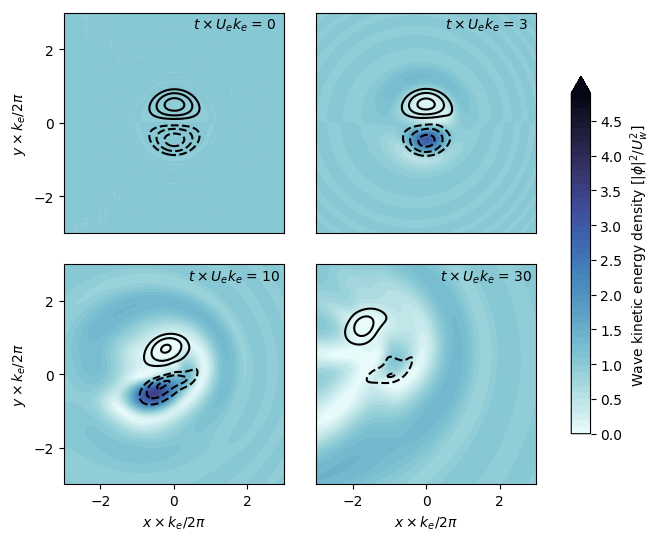
\includegraphics[width=.925\textwidth]{figs/fig1.png}
\caption{Snapshots of the Lamb-Chaplygin dipole solution with $\hslash \approx 1$
        and $\alpha \approx 3.75$. Colors represent wave kinetic energy density,
         $|\phi'|^2/U_w^2$.
        Contours represent potential vorticity, $q / (U_e k_e) = [
        -1.5,-0.5,1.5,0.5]$, with dashed lines showing negative values.
        These plots only show the central $(1/5)^2$
        of the simulation domain. (The supplemental material contains a video
        of the simulation.)}
\end{figure}

\begin{figure}
\label{stats_lamb}
\centering
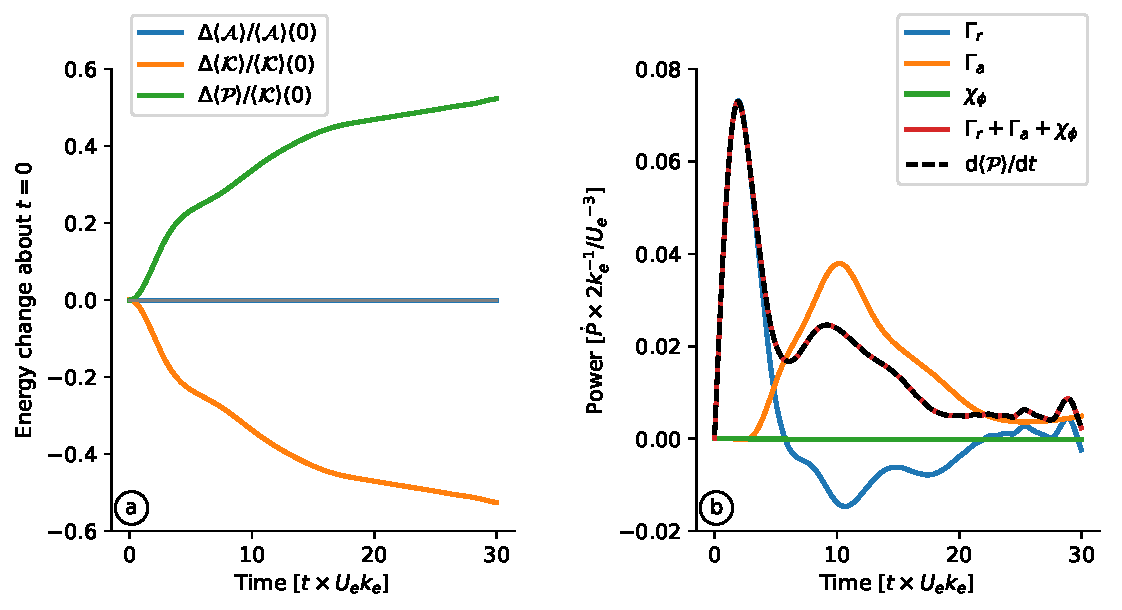
\includegraphics[width=1.\textwidth]{figs/fig2.pdf}
\caption{Statistics of the Lamb-Chaplygin dipole solution with $\hslash \approx 1$
        and $\alpha \approx 3.75$. (a) Energy change about initial condition.
        (b) Wave potential energy budget \eqref{Pw}. (c) Incoherent wave kinetic
        energy budget \eqref{Kiw}. (d) Coefficient of correlation between
        incoherent wave
        kinetic energy and geostrophic relative vorticity \eqref{corr_r}.
        }
\end{figure}

Because the advective conversion, $\Gamma_a$, remains positive for the duration
of the simulation, $\Gamma_a$ accounts for the bulk conversion of energy from
geostrophic flow to waves. Indeed, the time-integrated $\Gamma_a$ represents $77.5\%$
of total geostrophic kinetic energy change (Table \ref{table1}); the time-integrated
refraction conversion, $\Gamma_r$, represents $22.7\%$ of the geostrophic kinetic
energy changes. And direct dissipation and wave-dissipation source
(Appendix B) account for the residual changes ($<1\%$).

% adds table 1, which is an output of a python script
% This is preferable, on reproducibility grounds, than adding values manually.
\begin{table}
\begin{center}
\caption{The time-integrated budget of wave potential energy and quasigeostrophic                kinetic energy of the Lamb-Chaplygin dipole expirement. \label{table1}}
\begin{tabular}{cccc}
$\dot{P}_w$ budget & Rel. contribution ($\int\dot{P}_w \dd t/\Delta P_w dt$) & $\dot{K}_e$ budget & Rel. contribution ($\int\dot{K}_e \dd t/\Delta K_e$) \\
$\Gamma_r$ & 1.2 & -$\Gamma_r$ & -0.551 \\
$\Gamma_a$ & 2.148 & -$\Gamma_a$ & -0.987 \\
$-$ & $-$ & $\Xi_r$ & 0.855 \\
$-$ & $-$ & $\Xi_a$ & 0.022 \\
$\chi_\phi$ & -2.348 & $\epsilon_\psi$ & -0.338 \\
Res. & 0.0 & Res. & 0.0 \\
\end{tabular}
\end{center}
\end{table}


\clearpage
\section{Decaying Macroturbulence}

To study the energy exchanges between near-inertial waves and quasigeostrophic flow
in regime relevant to the ocean, we consider a barotropic turbulence flow that emerges from
random initial conditions integrated for 20 eddy turnover time units.
In other words, we first integrate the initial condition
\beq
\label{psi_init}
\psi \big(x,y, t \times U_e k_e = -20\big) = \sum_{k,l} |\hat{\psi}|\cos\left(k x + l y +
\chi_{k,l}\right)
\eeq
with waveless QG dynamics before introducing waves at $t\times U_e k_e = 0$.
In \ref{psi_init}, $\chi_{k,l}$ is a random phase uniformly distributed on $[0, 2\pi)$,
 and $|\hat\psi|$ is the streamfunction isotropic spectrum
\beq
\label{psih_mag}
|\hat{\psi}| = C \times \big\{|k|\,[1 + (|k|/k_e)^4]\big\}^{-1/2}\com
\eeq
with the wavenumber magnitude $|k|^2 = k^2 + l^2$. The prescribed initial energy
$U_e^2/2$ determines the constant C:
\beq
\label{ke_init}
\sum_{k,l} \underbrace{|k|^2 |\hat{\psi}|^2}_{\defn \cK_e} = \tfrac{1}{2}U_e^2\per
\eeq
The kinetic energy spectrum, $\cK_e$, peaks at the energy-containing scale $k_e^{-1}$.
At scales larger than $k_e^{-1}$, $\cK_e$ has a linear dependence on $|k|$,
whereas $\cK_e$ decays as $|k|^{-3}$ at scales smaller than $k_e^{-1}$. This red spectrum
ensures insignificant energy dissipation by the biharmonic diffusivity in \eqref{macroturb}.

 The evolution of a random initial condition constrained by the quasi-inviscid
 quasigeostrophic dynamics \eqref{macroturb} has been well studied, beginning
with \cite{fornberg1977}.
 Stirring of vorticity, $\lap \psi$, by the flow, $\psi$, transfers enstrophy towards
 small scales; energy flows to large
 scales. Most of enstrophy is dissipated within few eddy turnover time units, whereas
 kinetic energy is nearly conserved. Vorticity concentrates into localized
 structures: after 20 eddy turnover time units, the vorticity is well-organized
 into a sea of coherent vortices that form via like-sign vortex merging
 \citep[e.g., ][]{mcwilliams1984}.

 We add a perfectly coherent near-inertial oscillation \eqref{NIO} to the mature
 barotropic turbulence at $t \times U_e k_e = 0$. For all parameters considered
 in the remaining of this paper, there are no qualitative long-term differences
 between the solutions described below and results from introducing the waves
 at $t\times U_e k_e = -20$.

 \begin{figure}
 \label{snaps_turb}
 \centering
 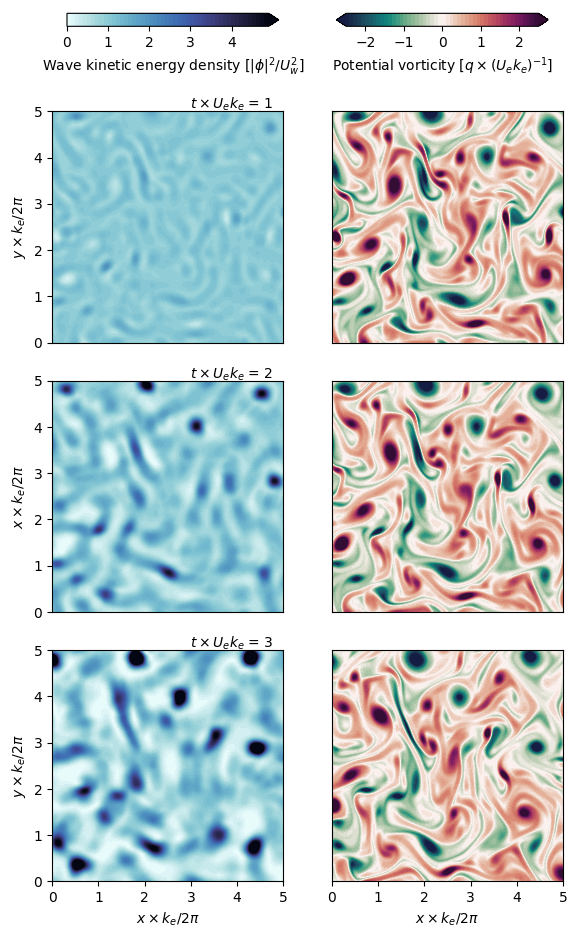
\includegraphics[width=.84\textwidth]{figs/fig3.png}
 \caption{Snapshots of the decaying turbulence solution with $\hslash \approx 1$
         and $\alpha \approx 1$. Left panels: wave kinetic energy density.
         Right panels: potential vorticity. These plots only show the bottom-left
        $(1/2)^2$ of the simulation domain. (The supplemental material contains a video
         of the simulation.)}
 \end{figure}

 \begin{figure}
 \label{stats_turb}
 \centering
 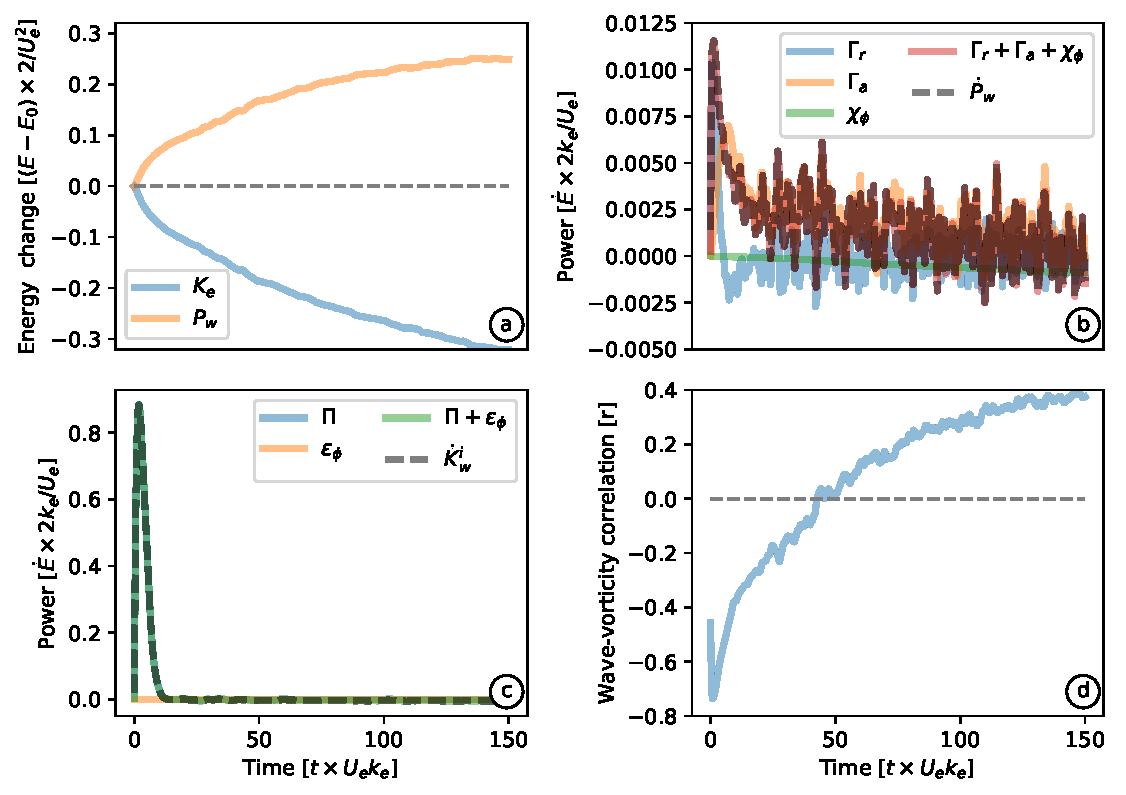
\includegraphics[width=1.\textwidth]{figs/fig4.pdf}
 \caption{Statistics of the decaying turbulence solution with $\hslash \approx 1$
         and $\alpha \approx 1$. (a) Energy change about initial condition.
         (b) Wave potential energy budget \eqref{Pw}. (c) Incoherent wave kinetic
         energy budget \eqref{Kiw}. (d) Coefficient of correlation between
         incoherent wave
         kinetic energy and relative vorticity \eqref{corr_r}.
         }
 \end{figure}

 % adds table 2, which is an output of a python script
 % This is preferable, on reproducibility grounds, than adding values manually.
 \begin{table}
\begin{center}
\caption{The time-integrated budget of wave potential energy and quasigeostrophic                kinetic energy of the decaying turbulence dipole expirement. \label{table2}}
\begin{tabular}{cccc}
$\dot{P}_w$ budget & Rel. contribution ($\int\dot{P}_w \dd t/\Delta P_w dt$) & $\dot{K}_e$ budget & Rel. contribution ($\int\dot{K}_e \dd t/\Delta K_e$) \\
$\Gamma_r$ & 0.002 & -$\Gamma_r$ & -0.002 \\
$\Gamma_a$ & 1.129 & -$\Gamma_a$ & -0.955 \\
$-$ & $-$ & $\Xi_r$ & 0.035 \\
$-$ & $-$ & $\Xi_a$ & -0.001 \\
$\chi_\phi$ & -0.131 & $\epsilon_\psi$ & -0.078 \\
Res. & 0.0 & Res. & -0.0 \\
\end{tabular}
\end{center}
\end{table}



 \begin{figure}
 \label{stats_turb_various}
 \centering
 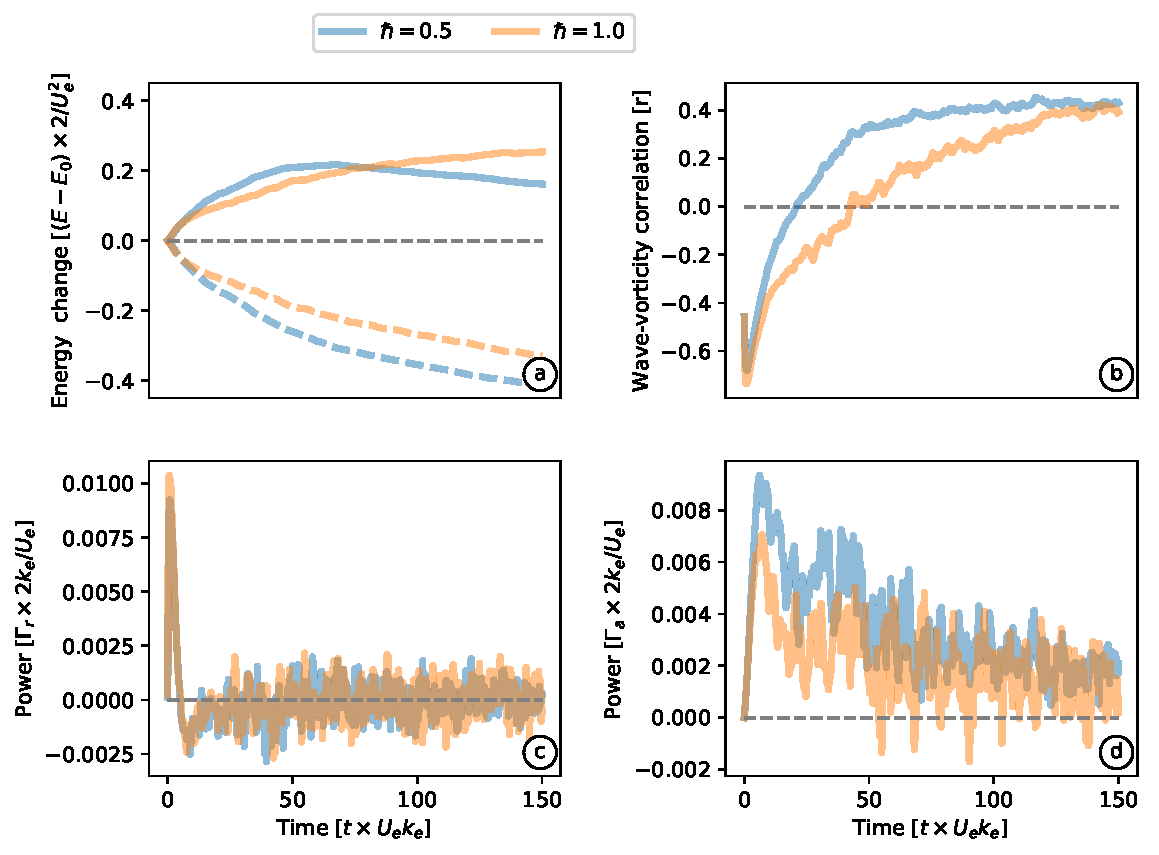
\includegraphics[width=1.\textwidth]{figs/fig5.pdf}
 \caption{Statistics of the decaying turbulence solution with $\alpha \approx 1$ and
         different dispersivities, $\hslash$. (a) Energy change about initial condition.
         (b) Coefficient of correlation between
         incoherent wave
         kinetic energy and relative vorticity \eqref{corr_r}. (c) Wave potential
         energy generation
         due to geostrophic refraction, $\Gamma_r$. (d) Wave potential energy generation due
         to geostrophic advection, $\Gamma_a$.
         }
 \end{figure}

 % \begin{figure}
 % \label{bulk_stats_turb_various}
 % \centering
 % 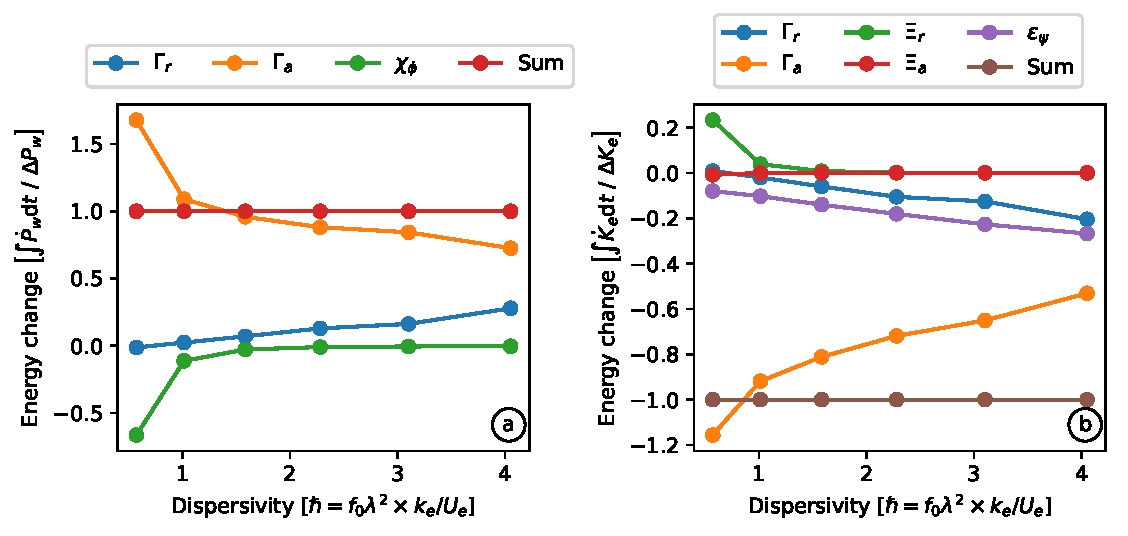
\includegraphics[width=1.\textwidth]{figs/fig7.pdf}
 % \caption{Energy budgets of the decaying turbulence solution $\alpha \approx 1$ and
 %         different dispersivities, $\hslash$. (a) Wave potential energy budget.
 %         (b) Geostrophic kinetic energy budget.
 %         }
 % \end{figure}


\subsection{Parameters for strong mid-latitude macroturbulence}

Consider strong mid-latitude macroturbulence, such as the Gulf Stream or Kuroshio
Extension. The choice of parameters, $U_e = 0.1$ m s$^{-1}$,
$f_0 = 1 \times 10^{-4}$ s$^{-1}$, $2\pi k_e^{-1} = 125$ km
gives a Rossby number $Ro \approx  0.05$. For reference, the eddy-turnover scale
is $(U_e k_e)^{-1}\approx 5.8\,\,\text{days}$. Strong near-inertial velocity
imparted by atmospheric storms, $U_w \sim \sqrt{2} U_e$, implies a wave amplitude
\beq
  \alpha \approx 0.1\per
\eeq
A near-inertial vertical wavelength of $\lambda_z = 2\pi/m = 300$ m \citep[e.g., ][]{alford_etal2016}
on a strongly stratified upper ocean, $N_0/f_0 = 100$, yields a dispersivity
\beq
  \hslash \approx 1.0 \per
\eeq

\subsection{Solutions for $\hslash = 1$ and $\alpha = 0.1$}

The decaying turbulence experiment qualitatively resembles the Lamb-Chaplygin solution.
Starting from a uniform wave field, refraction quickly concentrates the waves into
anticyclones. By
$t\times U_e k_e \approx 2$ there is a four-fold modulation of the wave kinetic
energy density on eddy scales (Figure \ref{snaps_turb}), reducing the lateral
coherence of the waves (Figure \ref{stats_turb}c). This initial wave concentration
into anticyclones is dramatic, $r < -0.75$, thereby causing a rapid wave potential
energy gain at the expenses of geostrophic kinetic energy loss
(Figure \ref{stats_turb}a).

The eddy-scale gradients of wave velocity support geostrophic advection and
wave dispersion. Indeed, the advective conversion, $\Gamma_a$, quicks off once
refraction imprints eddy scales on the wave field. Both advection and wave dispersion
reduce the wave concentration in anticyclones, and the refraction conversion,
$\Gamma_r$, decreases dramatically, reducing by half  at $t\times U_e k_e \approx 3$.
(Figure \ref{stats_turb}d). At this point, the $\Gamma_a$ takes over the total energy conversion. At later
evolution, $t\times U_e k_e > 5$ , the refraction conversion is small
in magnitude and oscillates about zero (Figure \ref{stats_turb}b).
But the large $\Gamma_a$ sustains the positive total energy conversion. The long-term
wave field has scales smaller than the eddies and no wave concentration into anticyclones
(Figure \ref{snaps_turb}).

Wave potential energy accounts for about $18\%$ of the bulk changes of geostrophic
kinetic energy (Table \ref{table2}). Advective conversion accounts for most of the
energy change, representing about 98$\%$ of the bulk energy conversion. Direct
dissipation accounts for about $11\%$ of the loss of geostrophic kinetic energy.
And the wave-dissipation source is significant: $\Xi_r$ contributes about $16\%$
of geostrophic kinetic energy gain.


\subsection{Varying wave dispersivity}


\subsection{Varying wave dissipation}


\section{Discussion}

% the advection sink rules
Both examples suggest that the advective conversion accounts for the bulk of geostrophic
kinetic energy sink --- and wave potential energy gain. But refraction is vital
to this problem with initially laterally coherent wave because it creates the
initial gradients of wave velocity that are then enhanced by geostrophic straining.
In more general problems, in which the waves initially have eddy scales, it's
likely that refraction catalyzes the geostrophic energy sink.

% concentration in anticyclones decreases with time

% we have focus
We have focused on the quasi-inviscid QG-NIW energy exchanges . Here, the small
small-scale dissipation contributes less than $10\%$ of the energy tendencies. But
increasing the wave dissipation changes the long-term, $t\times U_e k_e > 10$,
results qualitatively. The direct effects of wave dissipation
on the geostrophic kinetic energy budget --- via $\Xi$ --- also deserve further
study. We plan
to explore the role of wave dissipation using forced-dissipative solutions in a
future study.

% the decay of laterally coherent wave
The decay of a laterally coherent near-inertial oscillation due to refraction by
geostrophic flow is relevant for mixed-layer slab models used to estimate the work
imparted by wind into the near-inertial wave field \citep[e.g., ][]{alford2001}. Without further
assumptions, it is unclear if the effect of refraction is sign definite. If the
NIWs have initial larger scales than the geostrophic field, then refraction
generates eddy-scale perturbations, implying a reduction of lateral coherence
($\Pi > 0$). But it remains unclear if this transfer can be parameterized as a linear
damping.


%
% Acknowledgements
%
\vspace{1.cm}
This study was supported by the National Aeronautics and Space Administration
and the National Science Foundation financially via grants NNX16AO5OH and NSFXXX.

%
% Appendix
%

\appendix

\section{Details of the QG-NIW model}

\subsection{The \cite{xie_vanneste2015} model}
\cite{xie_vanneste2015} derive the QG-NIW model using a variational formulation
of the generalized Lagrangian mean (GLM) framework with Whitham averaging.
Following \cite{young_benjelloul1997}, Xie \& Vanneste write the
NIW velocity in complex form
\beq
u_w + \ii v_w = M_z \ee^{-\ii f_0 t}\per
\eeq
Their derivation recovers the wave equation that governs the
evolution of the NIW complex amplitude $M_z$,
\beq
M_{zzt} + \p_z \sJ(\psi,M_{z}) + \tfrac{\ii}{2}\left[\left(\frac{N^2}{f_0}+\psi_{zz}
\right)\lap M - 2 \nabla\psi_z\cdot\nabla M_z + M_{zz}(\lap\psi + 2 \beta y) \right] = 0 \com
\eeq
with the QG streamfunction $\psi(x,y,z,t)$. The QG flow evolves through stirring of QGPV
\beq
q_t + \sJ(\psi,q) = 0\per
\eeq
A fundamental difference to \cite{young_benjelloul1997} is that the QGPV in the
\cite{xie_vanneste2015} model contains quadratic wave terms
\beq
q = \nabla \psi + \left(\tfrac{f_0^2}{N^2}\psi_z\right)_z + \beta y +
    \tfrac{\ii}{2 f_0}\sJ(M_z^\star,M_z) + \tfrac{1}{4f_0}\left(
    2 |\nabla M_z|^2 - M_{zz}^\star\nabla M - M_{zz}\nabla M^\star\right)\com
\eeq
thus NIWs affect the QG flow.
The model of \cite{xie_vanneste2015}, with the potential vorticity that includes
wave terms, generalizes early ideas introduced by
 \cite{buhler_mcintyre1998}  to a setup that avoids spatial scale separation between
 geostrophic flow and waves, but restricts attention to near-inertial frequencies.
Using standard perturbation theory, \cite{wagner_young2016}
recovered and extended this coupled QG-NIW system.

The special family of solutions with barotropic, f-plane QG flow, uniform background
stratification, and single vertical mode NIW, $M_z = \ee^{\ii m z}\,\phi(x,y)$,
yields the reduced set of equations \eqref{macroturb}-\eqref{waves} used
in this paper.

\subsection{Wave self-interaction and frequency shift}
% To gain further insight into the dynamics, we decompose the balanced flow
% into `vorticity-induced' and `wave-induced' fields, $\psi = \psiq + \psiw$, where
% \beq
% \label{q_qw}
%     \lap\psiq = q\com\qquad\text{and}\qquad \lap\psiw =-\frac{1}{4f_0}\lap|\phi|^2
%      - \tfrac{\ii}{2f_0}\sJ(\phis,\phi)\per
% \eeq
% With the \eqref{q_qw} decomposition, the QGPV equation \eqref{macroturb} becomes
% \beq
% \label{lpsiq_t}
% \lap\psiq_t + \sJ(\psiq+\psiw,\lap\psiq) = 0\per
% \eeq
% In other words, the relative vorticity of the `vorticity-induced' flow changes
% due to advection by the total flow $\psiq+\psiw$. The wave equation satisfies
% \beq
% \label{waves2}
% \underbrace{\left(\p_t - \tfrac{\ii}{2} f_0\lambda^2\lap\right)\phi}_{\text{Lin.
% wave dynamics}} + \underbrace{\sJ(\psiw,\phi) +\tfrac{\ii}{2}\phi\lap\psiw}_{
% \text{Non-lin. wave dynamics}} +\,\, \underbrace{\sJ(\psiq,\phi)+\tfrac{\ii}{2}
% \phi\lap\psiq}_{\text{Adv./refrac. by } \psiq}  = 0\per
% \eeq
% From \eqref{q_qw}, the `wave-induced' streamfunction $\psiw$ is quadratic in $\phi$:
% \beq
% \label{psiw}
% \psiw = \tfrac{1}{4f_0}|\phi|^2 + \tfrac{\ii}{2f_0}\lap^{-1}\sJ(\phis,\phi)\com
% \eeq
% where $\lap^{-1}$ is the inverse of the Laplacian: $\lap^{-1}\lap f = f $.
%
% Together, equations \eqref{waves2}-\eqref{psiw} show the non-linear
% nature of the wave equation in this coupled QG-NIW model. In particular, the
% non-linear wave dynamics is cubic in wave amplitude.  Dropping these cubic
% wave terms yields a quasi-linear (QL) QG-NIW system. This
% QL system conserves the energy
% \beq
% E_{ql} \defn \la\half|\grad\psi^q|^2\ra + \la\grad\psi^q\cdot\grad\psi^w\ra +
%           \la\tfrac{\lambda^2}{4}|\grad\phi|^2\ra\per
% \eeq
% Note that   E = $E_{ql} + \la\half|\grad\psi^w|^2\ra$. Thus, the QL approximation
% is an intermediate model between the uncoupled QG-YBJ model ($\psi^w=0$)
% and the non-linear coupled QG-NIW model.

The the wave equation \eqref{waves} is non-linear because both $q$ and $\phi$
determine the flow $\psi$, which advects and refracts $\phi$. The wave contribution
to $\psi$ is quadratic in $\phi$ (cf. \eqref{qgpv}). Thus, the non-linear wave
dynamics in   \eqref{waves} is cubic in $\phi$.
To study these non-linear wave effects, we linearize the QG-NIW equations  about
 the exact solution
$\phi = \Phi = \text{constant}$ and $\psi = 0$, so that $q=0$. The QGPV
equation \eqref{macroturb} linearized about this state is trivial: $q_t = 0$,
 thus $q$ remains zero. Also,
\beq
\label{lin_q}
 \lap \psi = -\tfrac{\Phi}{2f_0}\lap\half(\phi + \phis)\com
\eeq
where $\phi$ represents the small departure about the constant $\Phi$, so that
the linearized wave equation becomes
\beq
\phi_t = \tfrac{\ii}{2}\left[\tfrac{\Phi^2}{2f_0}\lap\half(\phi+\phis) +
f_0\lambda^2\lap\phi\right] \per
\eeq
Recalling that $u_w + \ii v_w = \phi \ee^{\ii (mz -f_0 t)}$, we recast the wave
equation:
\beq
\left[\p_t^2 - \tfrac{1}{4}f_0\lambda^2\left(f_0\lambda^2+
\frac{\Phi^2}{2f_0}\right)\lap^2\right] v_w = 0\com
\eeq
where $\lap^2 = (\p_x^2 + \p_y^2)^2$. Hence, plane-wave solutions yield the
dispersion relation
\beq
\omega = \half f_0\lambda^2(k^2+l^2)\left[1+\half\tfrac{\Phi^2}{f_0^2\lambda^2}
\right]^{1/2}\com
\eeq
and we conclude that the wave self-interaction shifts the frequency by
\beq
\left[1+\half\tfrac{\Phi^2}{f_0^2\lambda^2}\right]^{1/2}-1\per
\eeq


\section{Details of the initial value problems}

\subsection{Small-scale dissipation}
To absorb the forward cascade of enstrophy, we add a biharmonic viscosity to the
potential vorticity equation \eqref{macroturb}
\beq
D_q = -\kappa_e \lap^2 q\com
\eeq
where $\lap^2 = (\p_x^2+\p_y^2)^2$.
Similarly, to prevent the development of very small scales, which may violate the
near-inertial approximation, we add a biharmonic viscosity in the wave equation
\eqref{waves}
\beq
D_\phi = -\kappa_w \lap^2 \phi\per
\eeq

The hyperviscous terms add small dissipation to the energy equations in
Section 2. The wave kinetic energy dissipation added to \eqref{action} is
\beq
\label{ep_phi}
\varepsilon_\phi \defn -\kappa_w\la|\lap\phi|^2\ra\per
\eeq
The kinetic energy dissipation \eqref{ep_phi} is associated only with the incoherent
wave field, $\phi'$, since $\lap\la\phi\ra = 0$. Hyperviscosity also dissipates
wave potential energy: the dissipation added to \eqref{Pw} is
\beq
\label{chi_phi}
\chi_\phi \defn -\kappa_w\tfrac{\lambda^2}{2}\la |\grad \lap\phi|^2 \ra \per
\eeq
Similarly, the geostrophic kinetic energy dissipation added to \eqref{Ke} is
\beq
\label{ep_q}
\varepsilon_q \defn \kappa_e \la \psi \lap q\ra = \kappa_e \la q \lap^2\psi\ra \com
\eeq
and the dissipation added to the potential enstrophy equation is
\beq
\label{chi_q}
\chi_q \defn -\kappa_e \la (\lap q)^2 \ra\per
\eeq
Wave dissipation also adds two extra terms to the geostrophic kinetic energy budget:
\beq
\label{xi}
\Xi = \underbrace{\tfrac{\kappa_w}{2 f_0}\left\la \lap\psi \half \left(\phis \lap^2\phi + \phi
\lap^2 \phis \right) \right\ra}_{\Xi_r} +
\underbrace{\tfrac{\kappa_w}{f_0}\left\la \tfrac{\ii}{2}\psi\left[\sJ(\phis,\lap^2\phi)-
\sJ(\phi,\lap^2\phis)\right]\right\ra}_{\Xi_a}\per
\eeq
The term $\Xi_r$ is easy to interpret: dissipation of wave kinetic energy,
$ \phis \lap^2\phi + \phi \lap^2\phis< 0$, in anticyclones, $\lap\psi <0 $, represents
a gain of geostrophic kinetic energy; this term is positive in all solutions of this paper.
The second term, $\Xi_a$, is obscure, but it is also positive in all solutions.
Hence, wave dissipation yields a gain of geostrophic kinetic energy.

In all solutions of initial value problems reported in this paper, the dissipative
terms \eqref{ep_phi}, \eqref{chi_phi}, \eqref{ep_q}, and \eqref{xi} account for
less than $10\%$ of the energy tendencies. The energy budgets
close within $10^{-5}\,\%$.

\subsection{Numerical methods}
We solve the QG-NIW system \eqref{macroturb}-\eqref{waves} using a standard
collocation Fourier spectral method.
In the pseudo-spectral spirit, we evaluate  the quadratic non-linearities in
physical space, and transform the product into Fourier space. We time march the
spectral equations
using an exponential time differencing method with a fourth order Runge-Kutta scheme
\citep[details in][]{kassam_trefethen2005}.

\subsection{Parameters}

\begin{table}
 \begin{center}
   \caption{Description of parameters of Lamb-Chaplygin simulation.}
   \label{parameters_lamb}
   \begin{tabular}{ c | c | c | c}
     \hline
      Parameter & Description & Value & Unit \\
      \hline
      $\mathsf{N}$   & Number of modes &  512 & -- \\
      $L_d$ & Domain size & $2\pi\times 200$ & km \\
      $2\pi k_e^{-1}$ & Dipole radius & $L/15 \approx 84$ & km \\
      $U_e$ & Dipole strength & $5\times 10^{-2}$ & m s$^{-1}$ \\
      $U_w$ & NIW speed & $5\times 10^{-1}$ & m s$^{-1}$ \\
      $(U_e k_e)^{-1}$ & Eddy turnover timescale & $\approx 3$ & days\\
      $N_0$ & Buoyancy frequency & $5 \times 10^{-3}$ & s$^{-1}$\\
      $f_0$ & Colioris frequency & 10$^{-4}$ & s$^{-1}$\\
      $2\pi$m$^{-1}$ & NIW vertical wavelength &  $325$ & m \\
      $\kappa_e$ & QGPV biharmonic viscosity & $5\times 10^{7}$  & m$^4$ s$^{-1}$\\
      $\kappa_w$ & NIW biharmonic viscosity & $ 5 \times 10^{7}$ & m$^4$ s$^{-1}$\\
   \end{tabular}
 \end{center}
\end{table}


%\begin{table}
%  \begin{center}
%    \label{parameters_description}
%    \caption{Description of parameters of numerical simulations.}
%    \begin{tabular}{ c | c | c }
%       Parameter & Description & Value \\ \hline
%       $\mathsf{N}$   & Number of modes &  512 \\
%       $L_d$ & Domain size & $2\pi\times 200$ km \\
%       $2\pi k_e^{-1}$ & Centroid wavelength & $2\pi\times 50$ km \\
%       $U_e$ & RMS velocity & $0.1$ m s$^{-1}$ \\
%       $U_w$ & NIW speed & $0.07 - 0.32$ m s$^{-1}$ \\
%       $N_0$ & Buoyancy frequency & 10$^{-2}$ s$^{-1}$\\
%       $f_0$ & Colioris frequency & 10$^{-4}$ s$^{-1}$\\
%       $2\pi$m$^{-1}$ & NIW vertical wavelength & $222 - 888$ m \\
%       $\kappa_e$ & QGPV biharmonic viscosity & $5\times 10^{7}$ m$^4$ s$^{-1}$\\
%       $\kappa_w$ & NIW biharmonic viscosity & $ 1 \times 10^{6}$ m$^4$ s$^{-1}$\\
%    \end{tabular}
%  \end{center}
%\end{table}

\subsection{Code and data}
Our python code that solves \eqref{macroturb}-\eqref{waves} on a doubly periodic domain
is available through a sustainable online repository
(\href{https://github.com/crocha700/niwqg}{https://github.com/crocha700/niwqg}).
The code is well tested and documented. We used version 0.1 in this study.

The data used to plot figures 1-6 are available on the repository of the paper:
\href{https://github.com/crocha700/RochaWagnerYoung_JFM}{https://github.com/crocha700/RochaWagnerYoung$\_$JFM}.
To ensure  reproduction and assist future studies, we also share the scripts that
setup and run the simulations and analyze the results of this paper.

\bibliographystyle{jfm}
% Note the spaces between the initials
\bibliography{RochaWagnerYoung}



\end{document}
